\section{Datasets}
\label{sec:datasets}

Data from VarDial 2020 and 2021 was acquired from a GitHub repository\footnote{\url{https://github.com/yvesscherrer/vardial-shared-tasks}} created by Yves Scherrer's, co-author of the winning solution for the \gls{acr:smg} task, both years. All but the test dataset has a ground truth associated with it, and I assume this unlabelled test dataset was used for a private leaderboard. The training, development, and test gold datasets have 22600, 3097, and 3068 labelled samples, respectively. \autoref{tbl:train-dataset} shows the first five rows of the training dataset. It was collected by \cite[2-3]{hovyCapturingRegionalVariation2018} using the (at the time) publicly available Jodel API.

\begin{table}
    \centering
    \begin{tabular}{l|rr|p{0.6\textwidth}}
        \toprule
          & lat   & lon  & text                                                                                                                                        \\
        \midrule
        0 & 47.22 & 7.43 & Dr Chester Bennington isch tot (pensive face)(pensive face)(pensive face) \#rip \#linkinpark Dr Manager heds bestätiged (expressionless)... \\
        1 & 46.86 & 8.21 & Mini Fründin hed Lust uf Doktorspieli gha... ... sie hocked jetzt sit 2 Stund...                                                            \\
        2 & 47.39 & 8.18 & Slayer isch besser. Det han ich gescht mini Drohne stiege lah (smiling face with smiling eyes) Cool was hesch f...                          \\
        3 & 47.37 & 8.78 & gaht au innere stund? bin grad am speck brate (nerd face) So langt chunsch ja münd eifach...                                                \\
        4 & 47.39 & 8.04 & sie: thy er: ? sie: thy= thank you er: player sege thx...                                                                                   \\
        \bottomrule
    \end{tabular}
    \caption{The first five rows of the training dataset}
    \label{tbl:train-dataset}
\end{table}

While Switzerland is a country with four official languages (Swiss-German, French, Italian, and Romansh Grishum), the dataset contains only Swiss-German Jodel messages, focusing on dialectal differences (the "Dial" in VarDial). This results in the heatmap in \autoref{fig:heatmap}.

\begin{figure}
    \centering
    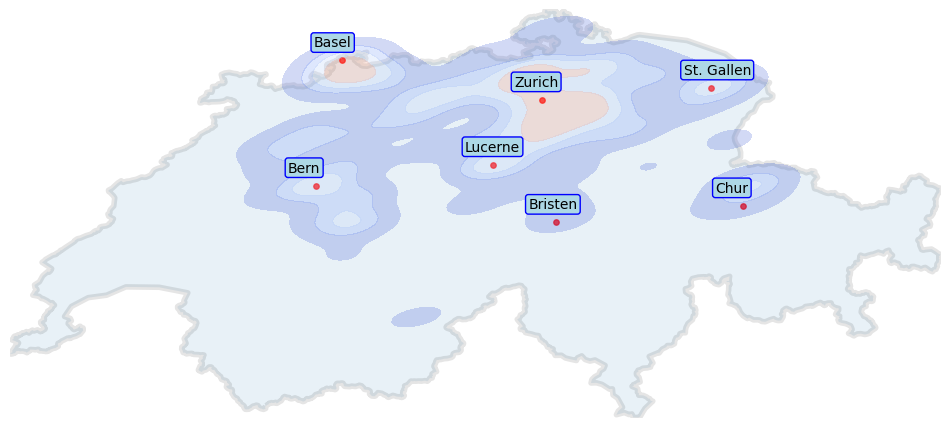
\includegraphics[width=\textwidth]{./figs/heatmap.png}
    \caption{Heatmap of the training data}
    \label{fig:heatmap}
\end{figure}

Attepmts were made to aquire a Norwegian dataset based on Norwegian Twitter/X messages using the method described in \cite{ljubesicTweetGeoToolCollecting2016} but due to recent changes in the Twitter/X API\footnote{\url{https://www.theverge.com/2023/5/31/23739084/twitter-elon-musk-api-policy-chilling-academic-research}} I was unable to do this. I also explored the possibility of using Norwegian Jodel messages but to my knowledge their API is no longer available to the public.